%!TEX program = lualatex
%!TEX encoding = UTF-8 Unicode  
%!TEX root = chapter07.tex  
\documentclass[main.tex]{subfiles}
\begin{document} 
%----------------------------------------------------------------------------------------
%	CHAPTER 08
%----------------------------------------------------------------------------------------
\cleardoublepage
\loadgeometry{marginlayout}  
\pagestyle{scrheadings} % Print headers again  
\KOMAoptions{
	headwidth=textwithmarginpar,
	headsepline=true,
	headsepline= 0.5pt,
	footwidth=textwithmarginpar,
}   
\onehalfspacing 
\setcounter{chapter}{6}

%----------------------------------------------------------------------------------------
%	COURS
%----------------------------------------------------------------------------------------

\chapter{Calculs algébriques (1) puissances et développements}
%Multiplication de puissances de même base 1h
%Multiplication et addition d'expressions 2h
%Identités remarquables 2h
%----------------------------------------------------------------------------------------
%	 
%----------------------------------------------------------------------------------------
%\newpage
\section[Puissances à exposants dans Z]{Puissances à exposants dans $\mathbb{Z}$}

\begin{marginfigure}
	\begin{tikzpicture} 
		\node[circle , draw , minimum size=2.3cm] (output)  {\Huge $2^4$};
		\node (puissance) [semithick, rectangle, draw,   below right=0.5cm and 0.2cm of output] {puissance};
		\node (exposant) [thin, rectangle, draw,   above right=0.1cm and 0.1cm of output] {exposant};
		\node (base) [thin, rectangle, draw,  below left=0.3cm and 0.1cm of output] {base};
		\draw[line width=0.8mm, -> ] (puissance) -- (output);
		\draw[line width=0.4mm, -> ] (base) --++ (0.9cm,0.9cm);
		\draw[line width=0.4mm, -> ] (exposant) --++ (-1.1cm,-0.7cm);
	\end{tikzpicture} 
	\caption{Vocabulaire}
	\label{fig:puissance}
\end{marginfigure}  
\begin{notation}
	Pour tout  $a\in\mathbb{R}^*$ et $n\in\mathbb{N}$ :
	\begin{multicols}{2}
		\begin{enumerate}[label={},leftmargin=*]
			\item  $a^0= 1$
			\item $a^1= a$
			\item $a^2= a\times a$
			\item $a^n = \underbrace{a \times a \times \ldots \times a}_{n\, \text{fois}}$ 
			\item $a^{-1}=\text{Inv  de $a$}=\frac{1}{a}$
			\item $a^{-2}=\text{Inv  de $a^2$}=\frac{1}{a^2}$
			\item  $a^{-n}=\text{Inv  de $a^n$}=\frac{1}{a^n}=\left(\frac{1}{a}\right)^n$   
		\end{enumerate}  
	\end{multicols}
\end{notation}
\begin{remark} Pour tout  $a\in\mathbb{R}^*$, et $n\in\mathbb{N}$ :  $\frac{1}{a^{-n}} = a^n$. \\
	En particulier  $\left(\frac{a}{b}\right)^{-n}=\left(\frac{b}{a}\right)^{n}$ et $\frac{a^{-n}}{b^{-m}}=\frac{b^m}{a^n}$.
\end{remark}
\begin{example} $
	2^5 ; \quad 3^{-2}; \quad -3^2; \quad (-3)^{-2};  \quad \left(\tfrac{5}{3}\right)^{-1};\quad \left(\tfrac{-9}{7}\right)^{-1};  \quad \left(\tfrac{2}{3}\right)^{-4} $
\end{example}
\begin{theorem}
	Pour tous  $m, n \in\mathbb{Z}$ et tous $a, b\in\mathbb{R}^*$ :
	\begin{description}
		\item[Multiplication de puissances de même base]  
		\marginnote{
			\begin{tBox}[frametitle=Règle 1, leftline=false]
				\og je multiplie des puissances, les bases sont les mêmes, j'ajoute les exposants \fg{}
			\end{tBox}
		}[-1cm] 
	\setlength{\abovedisplayskip}{3pt}
	\setlength{\belowdisplayskip}{3pt}
		\[ 
		a^m\times a^n   =a^{m+n} 
	 \qquad 
		\frac{a^m}{a^n}   =a^m\times \frac{1}{a^n} = a^{m-n}   
		\] 
		\item[Puissance d'une puissance]
		\setlength{\abovedisplayskip}{3pt}
		\setlength{\belowdisplayskip}{3pt}
		\[ 
		(a^n )^m  = a^{nm} 
		\] 
		\item[Multiplication de puissances de même exposant] 
		\marginnote{
			\begin{tBox}[frametitle=Règle 2, leftline=false]
				\og la puissance d'un produit est le produit des puissances \fg{}.
			\end{tBox}
		}[-1.5cm]
		\setlength{\abovedisplayskip}{3pt}
		\setlength{\belowdisplayskip}{3pt}
		\[ 
		(ab)^n = a^n b^n \qquad  \left(\frac{a}{b}\right)^n  = \frac{a^n}{b^n}
		\] 
		\marginnote{
			\begin{tBox}[frametitle=Règle 2 cas particulier, leftline=false]
				Pour tous réels $a\neq 0$ et $b\neq 0$  
				\begin{align*} 
					(ab)^2 &= a^2 b^2 \\
					\left(\frac{a}{b}\right)^2 &= \frac{a^2}{b^2} 
				\end{align*}  
			\end{tBox}
		}[-1cm] 
	\end{description}
\end{theorem} 
\begin{example} 
	Illustrer et justifier les simplifications des expressions suivantes sous la forme $a^n$ avec $a\in\mathbb{R}$   et $n\in\mathbb{Z}$
	\setlength{\abovedisplayskip}{3pt}
	\setlength{\belowdisplayskip}{3pt}
	\[
	3^4\times 5^4 ;\quad (-7)^3\times(-7)^{-5};\quad \frac{2^3}{2^{-2}};\quad (3^4)^7
	\]
\end{example}
%----------------------------------------------------------------------------------------
%	 
%----------------------------------------------------------------------------------------
%----------------------------------------------------------------------------------------
%	 EXERCICES
%----------------------------------------------------------------------------------------
\newpage 
\loadgeometry{widelayout}  
\pagestyle{scrheadings} % Print headers again  
\KOMAoptions{
headwidth=textwithmarginpar,
headsepline=true,
headsepline= 0.5pt,
footwidth=textwithmarginpar,
} 
\onehalfspacing
\subsection{Exercices : puissances à exposant entier}
\begin{eBox}
$a\neq0$,	$n>0$ : \hfill	$a^n= \underbrace{a \times a \times \ldots \times a}_{n\, \text{fois}}$ \hfill $a^{-n}=\frac{1}{a^n}=\left(\frac{1}{a}\right)^n$\hfill\null

\noindent Préciser la base en rajoutant des parenthèses !\\
 \begin{tikzpicture}
	\node[minimum size=3cm] (output) [thick, font=\fontsize{40}{0}\selectfont, thick] {$3a^4$};%circle , draw , 
	%	\node (puissance) [thick, rectangle, draw, font=\fontsize{10}{0}\selectfont, below right=0.3cm and 1.3cm of output] {puissance};
	\node (exposant) [thick, rectangle, draw, font=\fontsize{10}{0}\selectfont, above right=-0.2cm and 0.3cm of output] {exposant};
	\node (base) [thick, rectangle, draw, font=\fontsize{10}{0}\selectfont, below left=-0.5cm and -0.25cm of output] {ici la base est $a$};
	\node (sens) [thick, rectangle,   font=\fontsize{10}{0}\selectfont, below  =1.75cm  of exposant] {signifie $3\times a\times a\times a\times a$};
	%	\draw[line width=1mm, ->] (puissance) -- (output);
	\draw[line width=1mm, ->] (base) --++  (1.8cm,0.8cm);
	\draw[line width=1mm, ->] (exposant) --++ (-1.7cm,-0.8cm);
\end{tikzpicture}
\hfill 
\begin{tikzpicture}
	\node[ minimum size=3cm] (output) [thick, font=\fontsize{40}{0}\selectfont, thick] {$(3a)^4$}; %circle , draw ,
	%	\node (puissance) [thick, rectangle, draw, font=\fontsize{10}{0}\selectfont, below right=0.3cm and 1.3cm of output] {puissance};
	\node (exposant) [thick, rectangle, draw, font=\fontsize{10}{0}\selectfont, above right=-0.2cm and 0.3cm of output] {exposant};
	\node (base) [thick, rectangle, draw, font=\fontsize{10}{0}\selectfont, below left=-0.5cm and -0.25cm  of output] {ici la base est $3a$};
	\node (sens) [thick, rectangle,   font=\fontsize{10}{0}\selectfont,     below  =1.75cm  of exposant] {signifie $3a\times 3a\times 3a\times 3a $};
	%	\draw[line width=1mm, ->] (puissance) -- (output);
	\draw[line width=1mm, ->] (base) --++ (1.8cm,0.8cm);
	\draw[line width=1mm, ->] (exposant) --++ (-1.7cm,-0.8cm);
\end{tikzpicture}
\end{eBox}
\vspace{-0.5em} 

\begin{exercise}[\cancel{\faCalculator}]  Écrire sous forme d'une fraction irréductible ou un nombre décimal\hfill% \vspace{-1.0em}
	\begin{multicols}{2}
			\begin{enumerate}[label={}, leftmargin=*]
				\begin{spacing}{2.2}
				\item  $2^5=$\dotfill 
				\item $3^{-2}=$\dotfill
				\item $-3^{2}=$\dotfill
				\item $-3^{-2}=$\dotfill
				\item $(-3)^{2}=$\dotfill  
				\item $3- 4^1=$\dotfill
				\item $3 - 2^0=$\dotfill
				\item $3 - 5^{-1}=$\dotfill
				\item $2\times 10^{-2}=$\dotfill
				\item  $\left(\frac{5}{3}\right)^{-1}=$\dotfill
				\item  $\left(-\frac{9}{7}\right)^{-1}=$\dotfill
				\item $\left(\frac{5}{3}\right)^{-3}=\left(\qquad\rule{0pt}{1.2em}\right)^3=$\dotfill
				\item $\left(\frac{2}{3}\right)^{-4} =\left(\qquad\rule{0pt}{1.2em}\right)^4=$\dotfill
				\item $(99)^0=$\dotfill
				\item$\left(\numprint{0.7}\right)^{-1}= \left(\tfrac{7}{10}\right)^{-1}=$\dotfill
				\item$\left(\numprint{0.8}\right)^{-2}= \left(\tfrac{8}{10}\right)^{-2}=$\dotfill
				\item $\numprint{0.25}^{-1}=$\dotfill
				\item $\numprint{0.25}^{-2}=$\dotfill
				\item $\numprint{0.2}^{-1}=$\dotfill
				\item $\numprint{0.2}^{-2}=$\dotfill
			\end{spacing}
			\end{enumerate}\vspace{-0.5em}
	\end{multicols}  
\end{exercise}
 \begin{exercise}[\cancel{\faCalculator}]	Complétez par $>$ , $<$ ou $=$ :\hfill \vspace{-1.5em}
 	\begin{spacing}{2}
 		\begin{multicols}{5}
 			\begin{enumerate}[label={},leftmargin=*]  
 				\item $6^0\dotfill 0$
 				\item $5^{-1}\dotfill 1$
 				\item $2^1\dotfill 1$
 				\item $4^{-2}\dotfill 1$
 				\item $25^0\dotfill 0$
 				\item $1^{100}\dotfill 1$
 				\item $(-1)^{-1}\dotfill 0$
 				\item $10^{-2}\dotfill 1$
 				\item $\frac{1}{7^{-2}}\dotfill 1$ 
 				\item $(-3)^{-4}\dotfill 0$     
 			\end{enumerate}
 		\end{multicols}
 	\end{spacing}
 	\vspace{-1.5em}
 \end{exercise}
 \begin{exercise}[\cancel{\faCalculator}]\hfill \vspace{-0.5em}
 	\begin{spacing}{2}
 		%		\begin{multicols}{2}
 			\begin{enumerate}[label={\arabic*)},leftmargin=*]
 				\item $(-2)^{1}=$\dotfill$(-2)^{0}=$\dotfill $(-2)^{-1}=$\dotfill$(-2)^{-2}=$\dotfill$(-2)^{-3}=$\dotfill 
 				\item Sachant que $2^{15}=\numprint{32768}$, on peut dire $(-2)^{15}=$\dotfill  $2^{-15}=$\dotfill$(-2)^{-15}=$\dotfill 
 				\item Sachant que $4^5=1024$, on peut dire $(-4)^5=$\dotfill  $4^{-5}=$\dotfill$\left(\frac{1}{4}\right)^5=$\dotfill 
 			\end{enumerate}
 			%		\end{multicols} 
 	\end{spacing}
 	\vspace{-1em} 
 \end{exercise} 


%----------------------------------------------------------------------------------------
%	  
%----------------------------------------------------------------------------------------
\newpage 
\begin{eBox}
\parbox{0.40\linewidth}{
	\begin{tikzpicture}
		\node[circle , draw , minimum size=3cm] (output) [thick, font=\fontsize{40}{0}\selectfont, thick] {$3x^4$};
		%	\node (puissance) [thick, rectangle, draw, font=\fontsize{10}{0}\selectfont, below right=0.3cm and 1.3cm of output] {puissance};
		\node (exposant) [thick, rectangle, draw, font=\fontsize{10}{0}\selectfont, above right=0.1cm and 0.7cm of output] {exposant};
		\node (base) [thick, rectangle, draw, font=\fontsize{10}{0}\selectfont, below right=0.5cm and 0.25cm of output] {la base est $x$};
		\node (coefficient) [thick, rectangle, draw, font=\fontsize{10}{0}\selectfont, below left=0.5cm and 0.25cm of output] {coefficient est $3$};
		%		\node (sens) [thick, rectangle,   font=\fontsize{10}{0}\selectfont, below  =0.75cm  of output] {signifie $3\times a\times a\times a\times a$};
		%	\draw[line width=1mm, ->] (puissance) -- (output);
		\draw[line width=1mm, ->] (base)  --++  (-2.5cm,1.2cm);
		\draw[line width=1mm, ->] (exposant) --++ (-1.8cm,-1.0cm);
	\end{tikzpicture}
}\hfill 
\parbox{0.55\linewidth}{
	Dans $3x^4$ est un monôme en $x$.
	\begin{enumerate}[label=\textbullet]
		\item $x$ est la variable, elle est aussi la base de la puissance
		\item L'exposant $4$ est le degré du monôme.
		\item Le coefficient est $3$. 
	\end{enumerate} 
	$3x^4=3\times x\times x\times x \times x$ 
} 
%Le terme mônome est réservé aux cas d'exposant  positif.  : $3x^{-1}=\frac{3}{x}$.
\end{eBox}
 \begin{example}[multiplication et puissances de monômes] Simplifie :\hfill \vspace{-0.5em} 
	\begin{spacing}{2} 
		\begin{enumerate}[label={},leftmargin=*]
			\item $(2x^3)(4x^7)=2\times 4\times x^3x^7=8 x^{3+7}=8x^{10}$
			\item $\big(-3x^5\big)\big(6x\big)=-3\times 6\times x^5x=\dotfill$
			\item $\big(-x^2\big)^5=(-x^2) (-x^2) (-x^2) (-x^2) (-x^2) =\dotfill $
			\item  $\big(3x^5\big)^2 =\big(\qquad \big)\big(\qquad \big)=\dotfill$ 
		\end{enumerate}
	\end{spacing}	 \vspace{-1em} 
\end{example}


\begin{exercise} Simplifie les expressions suivantes.\hfill \vspace{-0.75em}
	\begin{multicols}{2}
		\begin{spacing}{2} 
			\begin{enumerate}[label={}, leftmargin=*]   
				\item $\big(x^2\big)\big(x^4\big)=\dotfill$
				\item $\big(7x^3\big)\big(2x^8\big)=\dotfill$
				\item $\big(-2x^5\big)\big(9x\big)=\dotfill$
				\item $\big(8x^3\big)\big(-2x^5\big)=\dotfill$ 
				\item $\big(-5x^6\big)^3 =\dotfill$
				\item $\big(2x^2\big)^6 =\dotfill $
				\item  $-(-3x)^2=\dotfill $
%				\item  $(2x)^2=\dotfill $
				\item  $(-xy)^2=\dotfill $
				\item  $(-x^2)^3=\dotfill $
				\item  $(3x)^3=\dotfill $
				\item  $(3x^2)^3=\dotfill $
				\item  $(-4xy^2)^3=\dotfill $
				\item  $-(4x)^2=\dotfill $
				\item  $-(-2x)^3=\dotfill $
				\item $\big(-x\big)^3\big(-x\big)^4=\dotfill$ 
				\item $-\big(-x\big)^2\big(x\big)^3=\dotfill$ 
			\end{enumerate}
		\end{spacing}%\vspace{-2em}
	\end{multicols}  
\end{exercise} 
\begin{exercise} Écrire les expressions suivantes comme puissances de $(x-y)$. On utilisera $y-x=-(x-y)$.\hfill \vspace{-0.75em}
%	\begin{multicols}{2}
		\begin{spacing}{2} 
			\begin{enumerate}[label={}, leftmargin=*]   
				\item $(x-y)^5\times (x-y)\times (x-y)^3=\dotfill $
				\item $(x-y)^5\times (x-y)^6\times (x-y)^7=\dotfill$ 
				\item $(y-x)^3=\big( -(x-y)\big)^3=\dotfill $
				\item $(y-x)^2= \dotfill $
				\item $(y-x)^2\times (x-y)=\big( -(x-y)\big)^2\times (x-y)=\dotfill $
				\item $(y-x)^3\times (x-y)^4=\dotfill $
				\item $(y-x)^2\times (x-y)^m=\dotfill $
			\end{enumerate}
		\end{spacing}%\vspace{-2em}
%	\end{multicols}  
\end{exercise} 
	 
%----------------------------------------------------------------------------------------
%	  
%----------------------------------------------------------------------------------------
\newpage 

 \begin{example}[division de puissances] Simplifie :\hfill \vspace{-0.5em} 
 	\begin{multicols}{2}
	\begin{spacing}{2.2} 
		\begin{enumerate}[label={},leftmargin=*]
			\item $3^5\divisionsymbol 3^2=3^5\times \frac{1}{3^2}=3^5\times 3^{-2}=3^3$
			\item  $8^7\divisionsymbol 8^{-4}=8^7\times \frac{1}{8^{-4}}=8^7\times 8^{4}=8^{11}$ 
			\item  $\frac{5}{5^2}=5\times 5^{-2}=5^{1-2}=5^{-1}=\dotfill$
			\item  $\frac{2^2}{2^{-3}}=2^2\times 2^{-(-3)}=2^{2+3}=2^{5}=\dotfill$
			\item  $\frac{2x^5}{3x^8}=\frac{2x^5x^{-8}}{3} =\frac{2x^{-3}}{3}=\dotfill$
			\item  $\frac{5x^3}{2x^{-2}}=\frac{5x^3x^{-(-2)}}{2} =\frac{5x^{5}}{2}=\dotfill$
		\end{enumerate}
	\end{spacing}	 \vspace{-1em} 
\end{multicols} 
\end{example}

\begin{exercise}[\cancel{\faCalculator}] Simplifiez les expressions suivantes et éliminer les exposants négatifs .\hfill \vspace{-1.0em}
	\begin{multicols}{2}
		\begin{spacing}{2.2}
			\begin{enumerate}[label={}, leftmargin=*]
				\item $\frac{4^{10}}{4^{3}}=$\dotfill  
				\item $\frac{3^{8}}{3^{2}}=$\dotfill 
				\item $\frac{3^{8}}{3^{8}}=$\dotfill 
				\item $\frac{3^5}{3}=$\dotfill 
%				\item $(-4)^{3}\divisionsymbol (-4)^{2}=$\dotfill 
%				\item $6^{4}\divisionsymbol 6^{8}=$\dotfill 
%				\item $\big(2^3\big)^{-2}\divisionsymbol \big(2^2\big)^{3}=$\dotfill 
				\item $4^{2}\divisionsymbol 4^{-3}=$\dotfill 
				\item $\frac{x^5}{x^2}=\dotfill$
				\item $\frac{x^3}{x^4}=\dotfill$
				\item $\frac{x^{-2}}{x^7}=\dotfill$
				\item $x^{-5}x^3=\dotfill$
				\item $x^{-2}x^{-4}x^5=\dotfill $
				\item $\frac{x^{16}}{x^{10}}=\dotfill$
				\item $x^2x^{-5}=\dotfill $
				\item $x^5x^{-3}x^{-4}=\dotfill $
				\item $\frac{x^7x^0}{x^{10}}=\dotfill $
			\end{enumerate}
		\end{spacing}\vspace{-0.5em}
	\end{multicols} 
\end{exercise} 
\begin{exercise}[\cancel{\faCalculator}] Simplifiez les expressions suivantes en éliminant les exposants négatifs .\hfill \vspace{-1.0em}
	\begin{multicols}{2}
		\begin{spacing}{2.2}	
			\begin{enumerate}[label={}, leftmargin=*]
				\item $\frac{x^7}{x^8  x^{-5}}=\dotfill$ 
				\item $x^4  (x^{-2})^3   x^5=\dotfill$  
				\item $\frac{x^4   x^{-1}}{x^8}=\dotfill$   
				\item $\frac{x^9x^{-2}}{x}=\dotfill$
				\item $\left(\frac{x}{2}\right)^3(5x^6)=\dotfill$
				\item $\big(x^{-4}x^3\big)^3=\dotfill$
				\item $\left(\frac{2x^2}{5}\right)^{-1}=\dotfill$
				\item $\left(\frac{5x^3}{2}\right)^{-2}=\dotfill$
		\end{enumerate}
	\end{spacing}\vspace{-0.5em}
\end{multicols} 
\end{exercise} 
\begin{example}  Simplifiez les expressions suivantes  et éliminer les exposants négatifs :\hfill \vspace{-0.5em} 
	\begin{multicols}{2}
		\begin{spacing}{2.2} 
			\begin{enumerate}[label={},leftmargin=*]
				\item $\frac{6xy^{-4}}{2x^{-2}y^2}=\frac{6}{2}\frac{x}{x^{-2}}\frac{y^{-4}}{y^2}=3x^{3}y^{-6}=\frac{3x^3}{y^6}$
				\item $\left(\frac{y}{3x^3}\right)^{-2}=\left(\frac{3x^3}{y}\right)^{2}=\frac{3x^3}{y}\times \frac{ 3x^3}{y}=\frac{9x^6}{y^2}$
			\end{enumerate}
		\end{spacing}	 \vspace{-1em} 
	\end{multicols} 
\end{example}
\begin{exercise}  Simplifiez les expressions suivantes  et éliminer les exposants négatifs .\hfill \vspace{-0.8em}
	\begin{multicols}{2}
		\begin{spacing}{2.2}	
			\begin{enumerate}[label={},leftmargin=*]
				\item $\frac{8x^3y^{-4}}{2x^{-5}y^5} =\dotfill $  
				\item $\frac{5xy^{-2}}{x^{-1}y^{-3}}=\dotfill $  
				\item $\left(\frac{y}{5x^{-2}}\right)^{-3}=\dotfill $  
				\item $\left(\frac{2x^{-1}y}{x^2y^{-3}}\right)^{-2}=\dotfill $  
				\item $\left(\frac{3x}{y^3}\right)^{-1}=\dotfill $ 
				\item $\left(\frac{x^{-1}y^{-2}}{x^{-5}y}\right)^{-1}=\dotfill $ 
			\end{enumerate}
		\end{spacing}\vspace{-0.5em}
	\end{multicols} 
\end{exercise} 
%\item $	\left(2x^{n+2}\right)^3$
% \item $\frac{\left(x \times x^n\right)^{2}}{x^{3n}}$ 
% \item $	\frac{x^5}{\left(x^3\right)^n} $ 
% \item $\left(\tfrac{1}{x}\right)^{2n}\times x^2 $  
\begin{example}  Simplifiez les fractions suivantes sous forme d'une somme de multiples d'une puissance de $x$ :\hfill \vspace{-0.5em} 
%	\begin{multicols}{2}
		\begin{spacing}{2.2} 
			\begin{enumerate}[label={},leftmargin=*]
				\item $\frac{2x^3-5x+5}{x}=2\frac{x^3}{x}-5\frac{x}{x}+\frac{5}{x}=2x^2-6+\frac{5}{x}$
				\item $\frac{5x^2-2x+1}{x^5}=\frac{5x^2}{x^5}-\frac{2x}{x^5}+\frac{1}{x^5}=5x^{-3}-2x^{-4}+x^{-5}=\frac{5}{x^3}-\frac{2}{x^4}+\frac{1}{x^5}$ 
			\end{enumerate}
		\end{spacing}	 \vspace{-1em} 
%	\end{multicols} 
\end{example}
\begin{exercise}Mêmes consignes. Eliminer les exposants négatifs :\hfill \vspace{-0.5em} 
	%	\begin{multicols}{2}
		\begin{spacing}{2.2} 
			\begin{enumerate}[label={},leftmargin=*]
				\item $\frac{-x^2+3x+1}{x}=\dotfill $
				\item $\frac{3x^2-x+2}{x^2}=\dotfill $
				\item $\frac{x^2-1}{x^4}=\dotfill $
				\item $\frac{x^3-x+2}{5x^3}=\dotfill $
			\end{enumerate}
		\end{spacing}	 \vspace{-1em} 
		%	\end{multicols}  
\end{exercise}
\begin{exercise}[\cancel{\faCalculator}] Simplifier les expressions suivantes sans utiliser la calculatrice. Montrer les étapes.\hfill \vspace{-0.5em} 
	%	\begin{multicols}{2}
		\begin{spacing}{2.2} 
			\begin{enumerate}[label={},leftmargin=*]
				\item $(-2)^{2022}+(-2)^{2023}=\dotfill$
				\item $2^{2024}-5\times 2^{2023}+6\times 2^{2022}=\dotfill$
				\item $3\times 2^{99}+6\times 2^{98}=\dotfill$
			\end{enumerate}
		\end{spacing}	 \vspace{-1em}  
\end{exercise}
\begin{exercise}[Je vérifie ma compréhension]  Entourez la ou les bonnes réponses.\hfill 

\noindent
\QCM[  Alterne,Reponses=4,Stretch=1.5,Largeur=2.5cm, AlphT]{ %Solution,Couleur=red!20, Titre,
	{$\frac{1}{10^{3}}=\ldots$}&{$10^{-3}$}&{$\numprint{0.0001}$}&{$\numprint{0.001}$}&{$1000$}&1,
	{$10\times 10^{-3}\times 10^5=\ldots$}&{$10^{-8}$}&{$10^{-15}$}&{$10^{2}$}&{$10^{3}$}&3,  
	{$5^{-3}\times 5\times 5^6=\ldots$}&{$5^4$}&{$5^{5}$}&{$5^{3}$}&{$5^{-16}$}&3, 
	{$\frac{7^{-5}}{7^{-9}}=\ldots$}&{$7^{-4}$}&{$7^{-14}$}&{$7^{14}$}&{$7^{4}$}&4, 
	{$x^5 + x^5=$}&{$2x^5$}&{$x^{10}$}&{$x^{25}$}&{$2x^{25}$}&1,  
	{$x^6=\ldots$}&{$(-x)^3\times (-x)^3$}&{$(-x)^2\times (-x)^4$}&{$(-x)^3\times (-x)^2$}&{$x^3\times x^2$}&,
	{Si $x^{n}=2$ alors $3x^{n+1}=$}&{$6$}&{$3x$}&{$6x$}&{$9x$}&2,
	{Si $x^{n+5}=5$ alors $x^{n+6}=$}&{$6$}&{$6x$}&{$5x$}&{$\frac{5}{x}$}&3,
	{Si $x^{n+3}=2$ alors $x^{n+2}=$ }&{$1$}&{$2x$}&{$x$}&{$\frac{2}{x}$}&4,
	{Si $x^{m}=a$ et $y^n=b$ alors}&{$x^{3m}=3a$}&{$y^{2n}=b^2$}&{\small$x^{3m}y^{2n}=ab^2$}&{\small$ x^{3m}y^{2n}=a^3b^2$}&4,
	{Si $x^{m}=a$ et $x^{n}=b$ alors $x^{m+2n}=$}&{$a+2b$}&{$2ab$}&{$(ab)^ 2$}&{$ab^2$}&1, 
	{$x^{2n+1}x^{5-n}=$}&{$x^{2n+6}$}&{$x^{n+6}$}&{$x^{2n-4}$}&{$x^{n-4}$}&2,
	{$\frac{x^{2n+1}}{x^{5-n}}=$}&{$x^{n+6}$}&{$x^{n+6}$}&{$x^{3n-4}$}&{$x^{n-4}$}&3,
} 	 
\end{exercise} 
%{$\frac{408^{409}}{408}=\ldots$}&{$408^{409}$}&{$409^{408}$}&{$408^{408}$}&{$407^{409}$}&3,  
%{$\frac{5^6}{5^{10}}=\ldots$}&{$5^4$}&{$5^{16}$}&{$5^{-4}$}&{$5^{-16}$}&3,  
%{$2\times 2^4=\ldots$}&{$4^4$}&{$4^5$}&{$2^4$}&{$2^{5}$}&1,  
%{$\frac{10^{-5}}{10^{7}}\times \frac{10^6}{10^7}=\ldots$}&{$10^{-13}$}&{$10^{-6}$}&{$10^{-48}$}&{$1^{-6}$}&3,  
%{$a^7\times a^7$}&{$2a^7$}&{$a^{14}$}&{$a^{49}$}&{$2a^{49}$}&2, 
%{$1=$}&{$10^0$}&{$10^0$}&{$10^0$}&{$10^0$}&

%----------------------------------------------------------------------------------------
%	 
%----------------------------------------------------------------------------------------

\newpage 
\loadgeometry{marginlayout}  
\pagestyle{scrheadings} % Print headers again  
\KOMAoptions{
	headwidth=textwithmarginpar,
	headsepline=true,
	headsepline= 0.5pt,
	footwidth=textwithmarginpar,
	paper=A4,
	paper=portrait,
}     

\onehalfspacing 
\newpage 
\section{Multiplier   des expressions algébriques}
\noindent 
Une \textbf{expression littérale} est une écriture mathématique qui contient des lettres appelées \textbf{variables}. 
 Une variable peut prendre des valeurs arbitraires.\sidenote{En mathématiques, on utilise certaines lettres pour différentes type de variables :
	\begin{itemize}[label=\textbullet,leftmargin=*]
		\item $n$ et $m$ ... pour les entiers positifs ou négatifs
		\item $x$, $y$ et $z$ pour des quantités inconnues.
		\item $a$, $b$ et $c$ sont réservés à des quantités connues.
\end{itemize}}.

\begin{definition}[Un monôme] est une expression de la forme $ax^n$ :
	\begin{enumerate}[label=\textbullet,leftmargin=*]
		\item $x$ est la variable
		\item $n\geqslant 0$ est le degré du monôme 
		\item $a$ est le coefficient.
	\end{enumerate}
	Les monômes de même degré sont dit \textbf{similaires}.
\end{definition}
\begin{example}\hfill 
	
	\tikzset{carre/.style={draw, rectangle , text width=1.75cm, align=center, minimum  height=2cm},
	}
	
	\tikzset{chose/.style={draw, rectangle , text width=2cm, align=center, minimum  height=1.5em},
	}
	\tikzset{cst/.style={draw, rectangle , text width=1.5em,   align=center, minimum  height=1.5em},
	}  
	\tikzset{coeff/.style={rectangle , text width=1.5em,   align=center, minimum  height=1.5em},
	}  
	\tikzset{sign/.style={ rectangle , text width=1.5em,   align=center, minimum  height=1.5em},
	}  
	\begin{tikzpicture}  
		\node[coeff] (coef1) [] {$5$}; 
		\node[carre] (xx1) [right=0.0em of coef1] {$x^2$}; 
		\node[sign] (pm1) [right=0.0em of xx1] {$+$};
		\node[coeff] (coef2) [right=0.0em of pm1] {$3$};  
		\node[chose] (x1) [right=0.0em of coef2] {$x$}; 
		\node[sign] (1)[right=0.0em of x1 ] {$+$}; 
		\node[cst] (2)[right=0.0em of 1 ] {$2$}; 
		%\node[chose] (x2)[below=0.0em of x1 ] {$x$}; 
	\end{tikzpicture}
	\begin{enumerate}[label=\textbullet]
		\item $2$ est le terme constant,  $3x$   le terme linéaire.  Il est \textbf{similaire}\sidenote{proportionnel à} à $x$.
%		\item $3x+2$ est une expression affine (de degré 1)
%		\item $5x^2$ est le monôme de degré 2. Il est similaire à $x^2$.
		\item $5x^2+3x+2$ est une expression \textbf{réduite ordonnée}.
	\end{enumerate} 
\end{example}
\begin{definition}
	Simplifier une expression algébrique revient à l'écrire sous forme réduite ordonnée.
\end{definition}
\marginnote{
	\begin{tBox}[leftline=false]
		interprétation simple : 
		$a$ paquets de $x$  + $b$ paquets de $x$   = $(a + b)$ paquets de $x$ !
	\end{tBox}
}  
\begin{tBox}[frametitle={Règle 1 : Axiome de distributivité}] 
	Pour tout réels $a$,$b$,$x\in\mathbb{R}$ :  
	$ 	(a+b)\times x = (a\times x)+(b\times x)  	$ 
\end{tBox}
\begin{tBox}[frametitle={Règle 2}] Pour tout réel $a$ :  
	$a \times (-1) = (-a)$
\end{tBox} 
\begin{definition}\textbf{Développer} est une activité qui consiste à exploiter les 2 règles précédentes jusqu'à plus possible pour écrire une expression égale sous forme d'une \textbf{somme de termes}.
\end{definition}
\begin{example}\hfill  
		\begin{enumerate}[label={$\Alph*=$}, leftmargin=*] 
			\item $-(a + b + c) = (-1) × (a + b + c) =  -a-b-c$
			\item $- (2x-5) = -2x+5   $ 
		\end{enumerate} 
\end{example}  
\begin{tBox}[frametitle={La double distributivité}]
	Pour tout réels $a$,$b$,$x, y\in\mathbb{R}$ :  
	\setlength{\abovedisplayskip}{3pt}
	\setlength{\belowdisplayskip}{3pt}
	$$
		(x + y)(a + b)  = x(a + b) + y(a + b)  = xa + xb + ya + yb
		$$
\end{tBox} 
\begin{example} Pour $x\in \mathbb{R}$. Développer :
\begin{multicols}{2}
	\begin{enumerate}[label={$\Alph*=$},leftmargin=*]
		\item   $-2(x-2)\times 5(x-3)$
		\item   $-2(x-2)+5(x-3)$
	\end{enumerate}
\end{multicols}
\end{example}

%----------------------------------------------------------------------------------------
%	 
%----------------------------------------------------------------------------------------

%----------------------------------------------------------------------------------------
%	EXERCICES
%----------------------------------------------------------------------------------------

\newpage 
\loadgeometry{widelayout}  
\pagestyle{scrheadings} % Print headers again  
\KOMAoptions{
	headwidth=textwithmarginpar,
	headsepline=true,
	headsepline= 0.5pt,
	footwidth=textwithmarginpar,
} 
\onehalfspacing
\subsection{Exercices : développer simplifier réduire et ordonner}
\begin{exercise}[Distributivité simple] \label{chap07:exo:simple1} Développer simplifier réduire et ordonner les expressions suivantes :
	\vspace{-0.5em}
\begin{multicols}{3}
	\begin{enumerate}[label={$\Alph*=$},leftmargin=*]
		\item$4\left(x+3\right)$
		\item$5\left(6x+1\right)$
		\item$2\left(3x-5\right)$
		\item$\left(4-3x\right)\times 2$
		\item$-\left(4-3x\right)$
		\item$5\left(2x+4x^2-2\right)$
		\item $3\left(5x+2\right)-4x$
		\item $3\left(4x+3\right)+2\left(5x-3\right)$
		\item $\left(5x+2\right)\times4-3\left(5x+6\right)$
	\end{enumerate}
\end{multicols} 
\end{exercise}
\begin{example}\hfill 
	
	
	
	\noindent\parbox{0.32\linewidth}{	
		$\begin{aligned}
			A (x)  &  =2(x+6)& &+2(x-3) \\
			&  = 2x+12\rule{0pt}{1.3em}&|&  \\
			&  =  \rule{0pt}{1.3em}&|&  \\
			&  =  \rule{0pt}{1.3em}     
		\end{aligned}$  	
	} 
	\hfill  \parbox{0.32\linewidth}{	
		$\begin{aligned}
			B (x)  &  =5(2x+6)& &-2(3x+4) \\
			&  = \rule{0pt}{1.3em}&|&  \\
			&  =  \rule{0pt}{1.3em}&|&  \\
			&  =  \rule{0pt}{1.3em}     
		\end{aligned}$ 
	} \hfill 
	\parbox{0.32\linewidth}{	
		$\begin{aligned}
			C (x)  &  =	4(5x+6)& &-5x(2x-3) \\
			&  = \rule{0pt}{1.3em}&|& \\
			&  =  \rule{0pt}{1.3em}&|&  \\
			&  =  \rule{0pt}{1.3em}     
		\end{aligned}$ 
	}  
	
\end{example}
\begin{exercise} \label{chap07:exo:simple2} Développer simplifier réduire et ordonner les expressions suivantes :
	\vspace{-0.5em}
	\begin{multicols}{3}
		\begin{enumerate}[label={$\Alph*=$},leftmargin=*]
			\item $2\left(x+4\right)+3\left(x+5\right)$
			\item $5\left(x+2\right)+4\left(x-2\right)$
			\item $3\left(4x+2\right)-2\left(x+2\right)$
			\item $7\left(x-2\right)-\left(3x+5\right)$
			\item $5\left(4x+2\right)-6\left(3x-1\right)$
			\item $3x\left(4x-5\right)-4\left(x^2+2\right)+2x$
		\end{enumerate}
	\end{multicols} 
\end{exercise}
\begin{example} Développer et simplifier réduire chacune l'expression suivante.
	
	\noindent\parbox{0.31\linewidth}{	
		$\begin{WithArrows}
			A(x)& = (2x+4)(x+5)\rule{0pt}{1.8em}  \\
			&=  \rule{0pt}{1.8em}  \\
			& =   \rule{0pt}{1.8em}  \\
			& =  \rule{0pt}{1.8em}   
		\end{WithArrows}$ 	
	} 
	\hfill 
	\parbox{0.31\linewidth}{	
		$\begin{WithArrows}
			B(x)& = (x-5)(2x+3)\rule{0pt}{1.8em}  \\
			&= \rule{0pt}{1.8em}  \\
			& =  \rule{0pt}{1.8em}  \\
			& =  \rule{0pt}{1.8em}    
		\end{WithArrows}$ 	
	}  \hfill  \parbox{0.31\linewidth}{	
		$\begin{WithArrows}
			C(x)& = (3x-4)(4x-3)\rule{0pt}{1.8em}  \\
			&= \rule{0pt}{1.8em}  \\
			& =  \rule{0pt}{1.8em}  \\
			& =  \rule{0pt}{1.8em}   
		\end{WithArrows}$ 	
	}  
\end{example}
\begin{exercise}[Distributivité double] \label{chap07:exo:double} Développer simplifier réduire et ordonner les expressions suivantes :
	\vspace{-0.5em}
	\begin{multicols}{3}
		\begin{enumerate}[label={$\Alph*=$},leftmargin=*]
			\item $ \left(2x+3\right)\left(x+5\right)$
			\item $ \left(2x+4\right)\left(x-3\right)$
			\item $ \left(x-5\right)\left(2x-4\right)$
			\item $ \left(2x+3\right)\left(2x-5\right)$
			\item $ \left(3x-4\right)\left(2x-3\right)$ 
			\item $ \left(3x-4\right)\left(3x+4\right)$ 
		\end{enumerate}
	\end{multicols} 
\end{exercise}
\begin{exercise}  Complétez les développements et simplifications suivantes :


\begin{spacing}{2}
	\noindent
	\parbox{0.48\linewidth}{
		$\begin{WithArrows}
			A(x)&=(x+\ldots)(x+\ldots) \\
			&=x^2+\ldots x + \ldots x + 24\\
			& =x^2+10x+24
		\end{WithArrows}$
	}
	\hfill
	\parbox{0.48\linewidth}{
		$\begin{WithArrows}
			B(x)&=(x+\ldots)(x+\ldots) \\
			&=x^2+8 x + \ldots x + 24\\
			& =x^2+\ldots x+\ldots
		\end{WithArrows}$
	}
	
	
	\noindent
	\parbox{0.48\linewidth}{
		$\begin{WithArrows}
			C(x)&=(x+\ldots)(x+\ldots) \\
			&=x^2+\ldots x + \ldots x + 18\\
			& =x^2+11x+18
		\end{WithArrows}$
	}	
	\hfill
	%\noindent
	\parbox{0.48\linewidth}{
		$\begin{WithArrows}
			D(x)&=(x+\ldots)(x+\ldots) \\
			&=x^2+\ldots x + 10 x + \ldots \\
			& =x^2+13x+\ldots
		\end{WithArrows}$
	}
	
	\noindent
	\parbox{0.48\linewidth}{
		$\begin{WithArrows}
			E(x)&=(x+\ldots)(x-\ldots) \\
			&=x^2-2x + \ldots x -14\\
			& =x^2+5 x-\ldots
		\end{WithArrows}$
	}
	\hfill
	\parbox{0.48\linewidth}{
		$\begin{WithArrows}
			F(x)&=(x+\ldots)(x+\ldots) \\
			&=x^2+\ldots x + \ldots x + \ldots\\
			& =x^2-14x+33
		\end{WithArrows}$
	} 

	\noindent
\parbox{0.48\linewidth}{
	$\begin{WithArrows}
		G(x)&=(x+\ldots)(x+\ldots) \\
		&=x^2+\ldots x + \ldots x +\ldots\\
		& =x^2+5 x +6
	\end{WithArrows}$
}
\hfill
\parbox{0.48\linewidth}{
	$\begin{WithArrows}
		H(x)&=(x+\ldots)(x-\ldots) \\
		&=x^2+\ldots x - \ldots x + \ldots\\
		& =x^2-25
	\end{WithArrows}$
} 
\end{spacing}
\end{exercise}
\vspace{-1em}
\begin{example} Développer et simplifier réduire chacune l'expression suivante.
	
	\noindent\parbox{0.48\linewidth}{	
		$\begin{WithArrows}
			A(x)& = (x-3)(x+1)(x+4) \rule{0pt}{1.8em}  \\
			&=  \rule{0pt}{1.8em}  \\
			& =   \rule{0pt}{1.8em}  \\
			& =  \rule{0pt}{1.8em}   \\
			& =  \rule{0pt}{1.8em}   \\
			&   
		\end{WithArrows}$ 	
	} 
	\hfill 
	\parbox{0.48\linewidth}{	
		$\begin{WithArrows}
			B(x)& = (x+2)(x-4)(x+2)\rule{0pt}{1.8em}  \\
			&= \rule{0pt}{1.8em}  \\
			& =  \rule{0pt}{1.8em}  \\
			& =  \rule{0pt}{1.8em}   \\
			& =  \rule{0pt}{1.8em}   \\
			&      
		\end{WithArrows}$ 	
	}  
\end{example}
\vspace{-1em}
\begin{exercise}[et si plus de facteurs ?]\label{chap07:exo:triple} Développer simplifier réduire et ordonner les expressions suivantes :
	\vspace{-0.5em}
	\begin{multicols}{3}
		\begin{enumerate}[label={$\Alph*=$},leftmargin=*]
			\item  $ x\left(x+2\right)\left(x+3\right)$
			\item  $ \left(x+1\right)\left(x+2\right)\left(x+2\right)$
			\item  $ \left(x+4\right)\left(x-2\right)\left(x+3\right)$
			\item  $ \left(x-2\right)^3$
			\item  $ \left(x-5\right)\left(x-1\right)\left(x+3\right)$ 
			\item  $ \left(2x+2\right)\left(3x-2\right)\left(x+3\right)$ 
		\end{enumerate}
	\end{multicols} 
\end{exercise}
\begin{exercise}[Mélange]\label{chap07:exo:melange} Développer simplifier réduire et ordonner les expressions suivantes :
	\vspace{-0.5em}
\begin{multicols}{2}
	\begin{enumerate}[label={$\Alph*=$},leftmargin=*]
		\item  $2\left(x-2\right)\left(x-4\right)-\left(2x+3\right)$  
		\item  $2x\left(x-2\right)+\left(x-4\right)-2\left(2x-3\right)$  
		\item  $-2\left(3x-4\right)\left(4x+2\right)-8\left(3-2x\right)$
		\item  $-\left(3x-2\right)\left(x-5\right)+\left(2x +3\right)\left(x-1\right)$
		\item  $5\left(x^2+4\right)\left(2x-3\right)-\left(x-5\right)\left(2x-3\right)$
		\item  $2\left(x+1\right)^2-\left(x-5\right)\left(x+5\right)$
	\end{enumerate}
\end{multicols} 
\end{exercise}
\begin{eBox}
	Une identité est une égalité toujours vraie. C'est une équation dont l'ensemble des solutions est $\mathbb{R}$.
\end{eBox}
\begin{exercise}\hfill 
	\begin{enumerate}[label=\alph*),leftmargin=*]
		\item Montrer que les valeurs $x=1$, $x=3$ et $x=5$ satisfont toutes l'équation $7(x-8)-3(x-20)=4(x+1)$
		\item Montrer que pour tout $x\in\mathbb{R}$   on a	$ 7(x-8)-3(x-20)=4(x+1) $
	\end{enumerate} 
\end{exercise}
\begin{exercise} \hfill 
	\begin{enumerate}[label=\alph*),leftmargin=*]
		\item Montrer que les valeurs $x=1$, $x=3$ et $x=5$ vérifient l'égalité $x^3-9x^2+23x=15$
		\item Montrer que l'égalité $ x^3-9x^2+23x=15$ n'est pas une identité. 
	\end{enumerate} 
\end{exercise}
\begin{exercise} Démontrer en développant \textbf{séparément} le membre de gauche et le membre de droite que pour tout $x\in\mathbb{R}$ on a $(2x-3)(5x-1)+3(x+5)(x-5) = x(13x-17)-72$.  
\end{exercise}

% 

%----------------------------------------------------------------------------------------
%	 
%----------------------------------------------------------------------------------------
 
\newpage 
\loadgeometry{marginlayout}  
\pagestyle{scrheadings} % Print headers again  
\KOMAoptions{
	headwidth=textwithmarginpar,
	headsepline=true,
	headsepline= 0.5pt,
	footwidth=textwithmarginpar,
	paper=A4,
	paper=portrait,
}     

\onehalfspacing 
\section{Identités remarquables} 
\begin{marginfigure}
	\begin{tikzpicture}[scale=0.80]
		\tkzSetUpPoint[size=3, fill=black]
		\tkzfctset{tan style/.style={->,>=latex, color=red, line width=1.2pt}}   
		\tkzSetUpLine[line width= 1.2pt, add=.5 and .5]  
		
		\tkzDefPoint(0,0){O}
		\tkzDefPoint(2.5,0){A}
		\tkzDefPoint(4,0){A'}
		\tkzDefSquare(O,A)\tkzGetPoints{B}{C}
		\tkzDefSquare(O,A')\tkzGetPoints{B'}{C'}
		\tkzDefPoint(4,2.5){D}
		\tkzDefPoint(2.5,4){D'}
		\tkzDrawPolygon(O,A,B,C)
		\tkzDefSquare(B,D)  \tkzGetPoints{C0}{B0}
		\tkzDrawPolygon(B,D,C0,B0)
		\tkzDrawPolygon(O,A',B',C')
		\tkzLabelSegment[below](O,A){$a$}
		\tkzLabelSegment[below](A',A){$b$}
		\tkzLabelSegment[left](O,C){$a$}
		\tkzLabelSegment[left](C,C'){$b$}
	\end{tikzpicture}
	\caption{Illustration géométrique du carré de la somme de nombres positifs $a\geqslant 0$ et $b\geqslant 0$}
	\label{chapitre02:figure:carresomme}
\end{marginfigure}   
\begin{theorem}[Carré de somme]
	Pour deux nombres $a\neq 0$ et $b\neq 0$ :
	\setlength{\abovedisplayskip}{3pt}
	\setlength{\belowdisplayskip}{3pt}
	\[
		(a+b)^2 = a^2+2ab+b^2  	(a-b)^2  = a^2-2ab+b^2   
	\]
\end{theorem}
\begin{proof}\hfill 

\noindent \parbox{0.45\linewidth}{	
	$\begin{WithArrows}
	(a+b)^2 &= (a+b)(a+b) \\
		&= \rule{0pt}{1.1em}\\
		& = \rule{0pt}{1.1em}  \\
		& = \rule{0pt}{1.1em}  
	\end{WithArrows}$ 	
}\hfill\parbox{0.45\linewidth}{	
	$\begin{WithArrows}
	(a-b)^2 &=  (a-b)(a-b) \\
		&= \rule{0pt}{1.1em}\\
		& = \rule{0pt}{1.1em}  \\
		& = \rule{0pt}{1.1em}  
	\end{WithArrows}$ 	
}  	  
\end{proof} 
\begin{example} \hfill \\
\noindent \parbox{0.45\linewidth}{	
	$\begin{WithArrows}
	A&= (2x-3)^2 \\
		&= \rule{0pt}{1.1em}\\
		& = \rule{0pt}{1.1em}  \\
		& = \rule{0pt}{1.1em}  
	\end{WithArrows}$ 	
}\hfill\parbox{0.45\linewidth}{	
	$\begin{WithArrows}
	B &=  (2x+3)^2 \\
		&= \rule{0pt}{1.1em}\\
		& = \rule{0pt}{1.1em}  \\
		& = \rule{0pt}{1.1em}  
	\end{WithArrows}$ 	
}   
\end{example}
%\begin{remark} Carrés de produits. Pour tous réels $a\neq 0$ et $b\neq 0$ :
%	\begin{align*} 
%		(ab)^2 &= a^2 b^2 & \left(\frac{a}{b}\right)^2 &= \frac{a^2}{b^2} 
%	\end{align*}  
%\end{remark}
\begin{marginfigure}
	\begin{tikzpicture}[scale=0.80] 
		\tkzSetUpPoint[size=3, fill=black]
		\tkzfctset{tan style/.style={->,>=latex, color=red, line width=1.2pt}}   
		\tkzSetUpLine[line width= 1.2pt, add=.5 and .5]  
		
		\tkzDefPoint(0,0){A}
		\tkzDefPoint(4,0){B}
		\tkzDefSquare(A,B)\tkzGetPoints{C}{D} 
		\tkzDefPoint(2.5,4){E} 
		\tkzDefSquare(C,E)\tkzGetPoints{F}{G}
		\tkzDrawPolygon[fill=gray!10](A,B,G,F,E,D) 
		\tkzDrawSegments[dashed](A,F)
		\tkzDrawSegments[dashed](C,E C,G)
		\tkzLabelSegment[above](C,E){$b$}
		\tkzLabelSegment[right](G,C){$b$}
		\tkzLabelSegment[left](A,D){$a$} 
		\tkzLabelSegment[above](A,B){$a$}  
		\begin{scope}[xshift=0cm, yshift=-3cm] 
			\tkzDefPoint(0,0){A}
			\tkzDefPoint(5.5,0){B}
			\tkzDefPoint(5.5,2.5){C}
			\tkzDefPoint(0,2.5){D}
			\tkzDefPoint(1.5,0){E}
			\tkzDefPoint(4,2.5){F}
			\tkzDrawPolygon[fill=gray!10](A,B,C,D) 
			\tkzDrawSegments[dashed](E,F)
			\tkzLabelSegment[right](B,C){$a-b$}
			\tkzLabelSegment[above](A,E){$b$} 
			\tkzLabelSegment[above](E,B){$a$} 
		\end{scope}
	\end{tikzpicture} 
	\caption{Illustration géométrique de la factorisation de la différence de deux carrés, avec $a\geqslant b \geqslant 0$}
	\label{chapitre02:figure:differencecarres}
\end{marginfigure}  
\begin{theorem}[Le produit de conjuqués]
	Pour tout réels $a$ et $b\in\mathbb{R}$ :
	\setlength{\abovedisplayskip}{3pt}
	\setlength{\belowdisplayskip}{3pt}
	\[
		(a+b)(a-b) =a^2- b^2  
	\]
	$(a-b)$ est le terme conjugué de $(a+b)$.\\
	$(a+b)$ est le terme conjugué de $(a-b)$
\end{theorem}
\begin{proof}\hfill
	
	\noindent \parbox{0.85\linewidth}{	
		$\begin{WithArrows}
			(a+b)(a-b) &=\\
			&= \rule{0pt}{1.1em}\\
			& = \rule{0pt}{1.1em}  \\
			& = \rule{0pt}{1.1em}  
		\end{WithArrows}$ 	
	} \\
	\null
\end{proof} 
\begin{example}\hfill 
	
	\noindent \parbox{0.45\linewidth}{	
		$\begin{WithArrows}
			A & =(2x-3)(2x+3) \\
			&= \rule{0pt}{1.1em}\\
			& = \rule{0pt}{1.1em}  \\
			& = \rule{0pt}{1.1em}  
		\end{WithArrows}$ 	
	}\hfill\parbox{0.45\linewidth}{	
		$\begin{WithArrows}
			B & =(\sqrt{5}+2)(\sqrt{5}-2) \\
			&= \rule{0pt}{1.1em}\\
			& = \rule{0pt}{1.1em}  \\
			& = \rule{0pt}{1.1em}  
		\end{WithArrows}$ 
		\marginnote{
			\begin{tBox}[leftline=false]
				$(ab)^2  = a^2 b^2$
			\end{tBox}
		}[0mm] 	
	}
\end{example}  

%----------------------------------------------------------------------------------------
%	EXERCICES
%----------------------------------------------------------------------------------------

\newpage 
\loadgeometry{widelayout}  
\pagestyle{scrheadings} % Print headers again  
\KOMAoptions{
	headwidth=textwithmarginpar,
	headsepline=true,
	headsepline= 0.5pt,
	footwidth=textwithmarginpar,
} 
\onehalfspacing
\subsection{Exercices : identités remarquables}


\begin{exercise}  Complétez les développements de carrés suivants à l'aide des identités remarquables :
	
	
	\begin{spacing}{2}
		\noindent
		\parbox{0.48\linewidth}{
			$\begin{WithArrows}
				A(x)&=(5x+3)^2 \\
				&=\big(\ldots x \big)^2+2\times \big(\ldots\ldots \big) \times \big(\ldots\ldots \big)  + \big(\ldots \big)^2\\
				&=\big(\ldots\big)^2 x^2+\ldots\ldots\ldots x  + \ldots\ldots\\
				& =\ldots x^2+\ldots x +\ldots 
			\end{WithArrows}$
		}
		\hfill
		\parbox{0.48\linewidth}{
			$\begin{WithArrows}
				B(x)&=(3x-4)^2 \\
				&=\big(\ldots x \big)^2+2\times \big(\ldots\ldots \big) \times \big(\ldots\ldots \big)  + \big(\ldots \big)^2\\
				&=\big(\ldots\big)^2 x^2+\ldots\ldots\ldots x  + \ldots\ldots\\
				& =\ldots x^2+\ldots x +\ldots 
			\end{WithArrows}$
		}
		
		
		\noindent
		\parbox{0.48\linewidth}{
			$\begin{WithArrows}
				C(x)&=(-x-2)^2 \\
				&=\big(\ldots x \big)^2+2\times \big(\ldots\ldots \big) \times \big(\ldots\ldots \big)  + \big(\ldots \big)^2\\
				&=\big(\ldots\big)^2 x^2+\ldots\ldots\ldots x  + \ldots\ldots\\
				& =\ldots x^2+\ldots x +\ldots 
			\end{WithArrows}$
		}	
		\hfill
		%\noindent
		\parbox{0.48\linewidth}{
			$\begin{WithArrows}
				D(x)&=(-3x+4)^2 \\
				&=\big(\ldots x \big)^2+2\times \big(\ldots\ldots \big) \times \big(\ldots\ldots \big)  + \big(\ldots \big)^2\\
				&=\big(\ldots\big)^2 x^2+\ldots\ldots\ldots x  + \ldots\ldots\\
				& =\ldots x^2+\ldots x +\ldots 
			\end{WithArrows}$
		}
		
		\noindent
		\parbox{0.48\linewidth}{
			$\begin{WithArrows}
				E(x)&=(\ldots x+\ldots)^2 \\
				&=\big(\ldots x \big)^2+2\times \big(\ldots\ldots \big) \times \big(\ldots\ldots \big)  + \big(\ldots \big)^2\\
				&=1^2 x^2+2\times \big(\ldots\ldots \big) \times 4  + 4^2\\
				& = x^2+\ldots x +16 
			\end{WithArrows}$
		}
		\hfill
		\parbox{0.48\linewidth}{
			$\begin{WithArrows}
				F(x)&=(2 x+\ldots)^2 \\
				&=\big(2 x \big)^2+2\times \big(\ldots\ldots \big) \times \big(\ldots\ldots \big)  + \big(\ldots \big)^2\\
				&=2^2 x^2+2\times \big(\ldots\ldots \big) \times \big(\ldots\ldots \big)   + 3^2\\
				& = 4x^2+18 x +9 
			\end{WithArrows}$
		} 
		
		\noindent
		\parbox{0.48\linewidth}{
			$\begin{WithArrows}
				G(x)&=(\ldots x-7)^2 \\
				&=\big(\ldots x \big)^2-\ldots\times \big(\ldots\ldots \big) \times \big(\ldots\ldots \big)  + \big( 7 \big)^2\\
				&=\ldots^2 x^2-\ldots \times \big(\ldots\ldots \big) \times 7  + 7^2\\
				& = 25x^2-\ldots x +49 
			\end{WithArrows}$
		}
		\hfill
		\parbox{0.48\linewidth}{
			$\begin{WithArrows}
				H(x)&=(\ldots x-\ldots)^2 \\
				&=\big(\ldots x \big)^2-\ldots\times \big(\ldots\ldots \big) \times \big(\ldots\ldots \big)  + \big( \ldots \big)^2\\
				&=\ldots^2 x^2-\ldots \times \big(\ldots\ldots \big) \times \ldots  + \ldots^2\\
				& = 4x^2-20 x +25 
			\end{WithArrows}$
		} 
	\end{spacing}
\end{exercise}\vspace{-1.5em}
\begin{exercise}[différence de carrés] Complétez :\vspace{-0.5em}
	\begin{spacing}{2}
		\begin{enumerate}[leftmargin=*,label={}]
			\item $(a+b)(a-b)=(\qquad )^2 - (\qquad)^2=\dotfill$ 
			\item $(x+2y)(x-2y)=(\qquad )^2 - (\qquad)^2=\dotfill$ 
			\item $(3x-4y)(3x+4y)=(\qquad )^2 - (\qquad)^2=\dotfill$ 
			\item $(2x+3y)(2x-3y)=$\dotfill 
			\item $(6-8x)(6+8x)=$\dotfill 
		\end{enumerate}
	\end{spacing}\vspace{-0.25em}
\end{exercise}
			
\begin{exercise}[\cancel{\faCalculator}] \hfill \vspace{-0.5em}
\begin{spacing}{2}
	\begin{enumerate}[leftmargin=*,label={\arabic*)}]
		\item Développer puis simplifier $(a+b)(a-2b)$ donne : \\
		(A) $a^2-2b^2$ \dotfill (B) $a^2+ab-2b^2$ \dotfill (C) $a^2-ab-2b^2$ \dotfill (D) $a^2+3ab-2b^2$
		\item Entourez les expressions qui sont égales à $a^2-b^2$ :\vspace{-0.5em}\\ 
		$(a+b)(a-b)$\hfill  
		$(-a-b)(-a+b)$\hfill 
		$(-a+b)(-a+b)$\hfill 
		$(-b-a)(b-a)$   
		\item Entourez les multiplications qui correspondent à une multiplication de conjuguées :\vspace{-0.5em}\\
		$(-x+2)(-x-2)$\hfill  
		$(x+2)(-x-2)$\hfill 
		$(x-2)(x+2)$\hfill 
		$(-x-2)(-x-2)$\\
		$(3-4x)(3+4x^2)$\hfill 
		$(3x-4)(-3x+4)$\hfill 
		$(3x+4)(-3x-4)$\hfill 
		$(3+4x^2)(3-4x^2)$
		\item 
		\noindent 
		\QCM[VF,Alterne,Stretch=1.0, Largeur=0.75cm]{% 
			{$(3a+2b)(3a-2b)=9a^2-4b^2$}&1,% 
			{$(-3a+2b)(-3a-2b)=9a^2-4b^2$}&1,% 
			{$(a+b+c)(a+b-c)=(a+b)^2-c^2$}&1,% 
			{$(a+b+c)(a-b+c)=(a+b)^2-c^2$}&2,% 
		}  
		\item Développer, simplifier et réduire les expressions suivantes :\vspace{-0.5em}
		\begin{enumerate}[label={},leftmargin=*]
			\item  $(1+x)(1-x)(1+x^2)=$\dotfill 
			\item  $(4+x^2)(2-x)(2+x)=$\dotfill 
			\item  $\big[(x-1)(x+1)\big]^2=$ \dotfill  
			\item  $(x-2y)^2(x+2y)^2=$ \dotfill 
			\item $(3x-y)^2-(3x+y)^2=$\dotfill 
		\end{enumerate}  
		\item En appliquant la formule des différences des carrés on peut calculer :
		\begin{enumerate}[label={},leftmargin=*]
			\item  $91\times 89  = (90+ \ldots\ldots)(90-\ldots\ldots) =\left( \qquad\qquad \right)^2- \left( \qquad\qquad \right)^2 = $\dotfill 
			\item $49.8\times 50.2  = (\ldots\ldots- \ldots\ldots)(\ldots\ldots+\ldots\ldots) =\left( \qquad\qquad \right)^2- \left( \qquad\qquad \right)^2 = $\dotfill 
			\item $99.9\times 100.1=\dotfill $ 
		\end{enumerate} 
	\end{enumerate}
\end{spacing}
\end{exercise} 
\vspace{-1.5em}
\begin{exercise} \label{chap07:exo:ir} Développer simplifier réduire et ordonner à l'aide d'identités remarquables adaptées :
	\vspace{-0.5em}
	\begin{multicols}{2}
		\begin{enumerate}[label={$\Alph*=$},leftmargin=*]
			\item $(3x+5)^2 $    
			\item $(3x+5)(3x-5) $    
			\item $\left(\frac{3}{4} x-\frac{4}{5}\right)\left(\frac{3}{4}x+\frac{4}{5}\right) $    
			\item $2(4x-3)^2$  
			\item $-(6x-5)(6x+5)$
			\item  $(6x+9)^2-(x-5)(x+5)$ 
			\item $(5x+2)^2-(2x+3)(2x-3)$
			\item  $(3x+2)(3x-2)- 2(x-5)^2$     
		\end{enumerate}
	\end{multicols} 
\end{exercise} 
\begin{exercise}\hfill \\
	 Montrer que pour tout $x\in\mathbb{R}$ on a :  $(3x -5)^2 -49=9(x-4)\left(x+\frac{2}{3}\right)$.
\end{exercise}
\begin{exercise}\hfill \\
	 Montrer que pour tout $x\in\mathbb{R}$ on a :  $−2(x − 1)^2 + 8 =-2(x-3)(x+1)$.
\end{exercise}
\begin{exercise} \hfill \\
	Montrer que pour tout $x\in\mathbb{R}$ on a :  $3(2x +1)^2 -48 = 12\left(x+\frac{5}{2}\right)\left(x-\frac{3}{2}\right)$.
\end{exercise} 
\begin{exercise} \hfill \\ 
	Trouver deux nombres $a$ et $b$ tel que pour tout $x\in\mathbb{R}$, $(x+a)^2-b=x^2+22x+71$.
\end{exercise}

\begin{exercise}\label{chap07:exo:equ01} \hfill \\
	Résoudre dans $\mathbb{R}$ l'équation $15(x+2)(x-2)-3(2x+1)(2x-1)=(x-2)(3x+1)$, inconnue $x$.\\
	\emph{Indication : développer simplifier les deux membres}
\end{exercise}
\begin{exercise}\label{chap07:exo:equ02} \hfill \\
	Résoudre dans $\mathbb{R}$ l'équation $(3x+1)(3x-1)+2(x+2)(x-2)=11(x+1)(x-3)$, inconnue $x$.
\end{exercise}
\begin{exercise}\hfill \\ 
Une pelouse carrée de côté $am$. On agrandi ses côtés nord et sud de $3~$m, et on réduit ses côtés est et ouest de $3~$m. La nouvelle aire de la pelouse est-elle supérieure ou inférieur à l'aire de départ ? Préciser la différence.
\end{exercise}
\begin{exercise}\hfill 
	
	\noindent\parbox{0.3\linewidth}{
		\begin{tikzpicture}[scale=1]
			\def \a{1.5};
			\def \b{2.5}; 
			\tkzDefPoint(0,0){O}
			\tkzDefPoint(\b,0){A1}
			\tkzDefPoint(\a+\b,0){A2}
			\tkzDefPoint(\a+\b,\a){B1}
			\tkzDefPoint(\a+\b,\a+\b){B2}
			\tkzDefPoint(\a,\a+\b){C1} 
			\tkzDefPoint(0,\a+\b){C2}
			\tkzDefPoint(0,\b){D1} 
			\tkzDrawPolygon[ line width=1.2pt,fill=gray!05](O,A2,B2,C2)
%			\tkzDrawPolygon[ line width=1.2pt,fill=gray!05](A1,A2,C2,C1)
%			\tkzDrawPolygon[ line width=1.2pt,fill=gray!05](D1,C2,D2,D3)
%			\tkzDrawPolygon[ line width=1.2pt,fill=gray!05](B2,E1,E2,E3)
		\tkzDrawPolygon[ line width=1.2pt,fill=gray!75](A1,B1,C1,D1)
			%			\tkzDrawSegments[dashed,line width=1.2pt](A1,B2 A1,C2 C2,D3 B2,E2)
			
			
			\tkzDrawSegment[dim={\small $b$,-10pt,}](O,A1)
			\tkzDrawSegment[dim={\small $b$,10pt,}](C1,B2)
			
			\tkzDrawSegment[dim={\small $a$,-10pt,}](A1,A2)
			\tkzDrawSegment[dim={\small $a$,-10pt,}](A2,B1)
%			
			\tkzDrawSegment[dim={\small $b$,-10pt,}](B1,B2)
			\tkzDrawSegment[dim={\small $a$,-10pt,}](C1,C2)
%			
			\tkzDrawSegment[dim={\small $a$,-10pt,}](C2,D1)
			\tkzDrawSegment[dim={\small $b$,-10pt,}](D1,O) 
			
		\end{tikzpicture}
	}\hfill
	\parbox{0.65\linewidth}{
		Justifier que l'aire de la partie grise du carré ci-contre est égale à $2ab$.
	}
\end{exercise}
\begin{exercise}\hfill 
	
	\noindent\parbox{0.3\linewidth}{
		\begin{tikzpicture}[scale=.8]
			%			\tkzInit[xmin=-1.0,ymin=-1.0,xmax=6.5,ymax=2.8]
			%			\tkzClip
			\tkzDefPoint(0,0){A} \tkzDefPoint(5,0){C}
			\tkzDefTriangle[two angles = 27 and 90](A,C)\tkzGetPoint{B}
			\tkzDrawPolygon[line width=1.2pt](A,B,C) 
			\tkzLabelSegment[below](A,C){$2$}
			\tkzLabelSegment[right](B,C){$x-\frac{1}{x}$} 
			\tkzLabelSegment[above left](A,B){$x+\frac{1}{x}$} 
		\end{tikzpicture} 
	}\hfill
	\parbox{0.65\linewidth}{
		Soit $x>1$. 
		\begin{enumerate}[leftmargin=*,label=\arabic*)] 
			\item Développer simplifier et réduire $\left(x+\frac{1}{x}\right)^2$ et $\left(x-\frac{1}{x}\right)^2$ .
			\item Montrer que pour tout $x>1$, le triangle ci-contre est rectangle.
		\end{enumerate}
	}
\end{exercise}

\begin{exercise}\hfill 
	
	\noindent\parbox{0.3\linewidth}{
		\begin{tikzpicture}[scale=1]
			\def \b{1.5};
			\def \a{2.5}; 
			\tkzDefPoint(0,0){O}
			\tkzDefPoint(\a,0){A1}
			\tkzDefPoint(\a+\b,0){A2}
			\tkzDefPoint(\a,\b){B1}
			\tkzDefPoint(0,\b){B2}
			\tkzDefPoint(\a,\a){C1}
			\tkzDefPoint(\a+\b,\a){C2}
			
			\tkzDefPoint(\b,\a){D1}
			\tkzDefPoint(\a+\b,\a+\b){D2}
			\tkzDefPoint(\b,\a+\b){D3}
			
			\tkzDefPoint(\b,\b){E1}
			\tkzDefPoint(\b,\a+\b){E2}
			\tkzDefPoint(0,\a+\b){E3}
			\tkzDrawPolygon[ line width=1.2pt,fill=gray!75](O,A1,B1,B2)
			\tkzDrawPolygon[ line width=1.2pt,fill=gray!75](A1,A2,C2,C1)
			\tkzDrawPolygon[ line width=1.2pt,fill=gray!75](D1,C2,D2,D3)
			\tkzDrawPolygon[ line width=1.2pt,fill=gray!75](B2,E1,E2,E3)
			\tkzDrawPolygon[ line width=1.2pt,fill=white](B1,C1,D1,E1)
			%			\tkzDrawSegments[dashed,line width=1.2pt](A1,B2 A1,C2 C2,D3 B2,E2)
			
			
			\tkzDrawSegment[dim={\small $\frac{1}{x}$,-15pt,}](O,A1)
			\tkzDrawSegment[dim={\small $x$,15pt,}](O,B2)
			
			\tkzDrawSegment[dim={\small $x$,-15pt,}](A1,A2)
			\tkzDrawSegment[dim={\small $\frac{1}{x}$,-15pt,}](A2,C2)
			
			\tkzDrawSegment[dim={\small $\frac{1}{x}$,-15pt,}](D2,D3)
			\tkzDrawSegment[dim={\small $x$,-15pt,}](C2,D2)
			
			\tkzDrawSegment[dim={\small $\frac{1}{x}$,-15pt,}](E2,E3)
			\tkzDrawSegment[dim={\small $x$,15pt,}](B2,E3) 
			
		\end{tikzpicture}
	}\hfill
	\parbox{0.65\linewidth}{
		Les 4 rectangles ci-contre sont égaux. 
		\begin{enumerate}[leftmargin=*,label=\arabic*)] 
			\item Développer simplifier et réduire $\left(x+\frac{1}{x}\right)^2$.
			\item En déduire que pour tout $x>0$,  $ x+\frac{1}{x}>2$
			\item Expliquer pourquoi l'inégalité précédente peut être illustrée par le graphique ci-contre.
		\end{enumerate}
	}
\end{exercise}


\begin{exercise}[]\hfill 

\noindent
\parbox{0.48\linewidth}{
\begin{enumerate}[label=\arabic*), leftmargin=*]
\item Développer simplifier et réduire 
\setlength{\abovedisplayskip}{3pt}
\setlength{\belowdisplayskip}{3pt}
$$\left(x+\frac{m}{2}\right)^2-\left(\frac{m}{2}\right)^2$$ 
\item Expliquer pourquoi l'identité précédente peut être illustrée par le graphique ci-contre.
\end{enumerate}  
}\hfill
\parbox{0.50\linewidth}{	 
	%\begin{figure*}[!h]
	\begin{tikzpicture}[scale=1.0] 
		\tkzSetUpPoint[size=3, fill=black]
		\tkzfctset{tan style/.style={->,>=latex, color=red, line width=1.2pt}}   
		\tkzSetUpLine[line width= 1.2pt, add=.5 and .5] 
		\def\a{3.8}
		\def\b{2.37}
		
		\tkzDefPoint(0,0){A} 
		\tkzDefPoint(\a,0){B} 
		\tkzDefPoint(\a,\b){C} 
		\tkzDefPoint(0,\b){D} 
		\tkzDrawPolygon[fill=gray!10](A,B,C,D)
		%		
		\tkzDefPoint(\b,0){E}
		\tkzDefPoint(\b,\b){F}
		%		
		\tkzDefPoint(0.5*\a+0.5*\b,0){G}
		\tkzDefPoint(0.5*\a+0.5*\b,\b){H}
		\tkzDrawLine[thin, dashed](G,H)
		
		\tkzDrawSegment[dim={\scriptsize $x$,+20pt,left=2pt}](A,D)
		\tkzDrawSegments[dashed](E,F)
		\tkzDrawSegment[dim={\scriptsize $x$,-20pt,below=3pt}](A,E)
		\tkzDrawSegment[dim={\scriptsize $m$, -20pt,below=3pt}](E,B)
		\tkzMarkSegments[mark=s||](E,G G,B C,H H,F)
		%		\tkzDrawPolygon[fill=gray!20](I,J,C,H)  
		%		\tkzLabelPoint[above left](A){\scriptsize$A$}
		%		\tkzLabelPoint[above right](B){\scriptsize$B$} 
		%		\tkzLabelPoint[below right](C){\scriptsize$C$} 	
		%		\tkzLabelPoint[below](D){\scriptsize$D$} 
		%		\tkzLabelPoint[above](E){\scriptsize$E$} 
		%		\tkzLabelPoint[below](F){\scriptsize$F$} 
		%		\tkzLabelPoint[above](G){\scriptsize$G$} 
		%		\tkzLabelPoint[below](H){\scriptsize$H$}  
		%		\tkzLabelPoint[left](I){\scriptsize$I$} 
		%		\tkzLabelPoint[right](J){\scriptsize$J$} 
		
		\begin{scope}[xshift=5.5cm] 
			
			\tkzDefPoint(0,0){A} 
			\tkzDefPoint(\b,0){B} 
			\tkzDefPoint(\b,\b){C} 
			\tkzDefPoint(0,\b){D} 
			\tkzDefPoint(0.5*\a+0.5*\b,0){G}
			\tkzDefPoint(0.5*\a+0.5*\b,\b){H}
			\tkzDefPoint(\b,0.5*\a+0.5*\b){E}
			\tkzDefPoint(0,0.5*\a+0.5*\b){F}
			\tkzDrawPolygon[fill=gray!10](A,G,H,C,E,F)
			\tkzDrawSegments[dashed](B,C C,D)
			\tkzMarkSegments[mark=s||](B,G C,H C,E F,D)
			\tkzDrawSegment[dim={\scriptsize $x$,+20pt,left}](A,D)
			\tkzDrawSegment[dim={\scriptsize $\tfrac{m}{2}$,+20pt,left}](D,F)
			
			
			\tkzDefPoint(0.5*\a+0.5*\b,0.5*\a+0.5*\b){I}
			\tkzDrawSegments[dashed](H,I I,E)
		\end{scope}
	\end{tikzpicture}
	%\end{figure*} 
}
\end{exercise}  
  

	
\begin{exercise}\hfill 
	
	\noindent\parbox{0.3\linewidth}{
		\begin{tikzpicture}[scale=1]
			\def \b{1.8};
			\def \a{2.5}; 
			\tkzDefPoint(0,0){O}
			\tkzDefPoint(\a,0){A1}
			\tkzDefPoint(\a+\b,0){A2}
			\tkzDefPoint(\a,\b){B1}
			\tkzDefPoint(0,\b){B2}
			\tkzDefPoint(\a,\a){C1}
			\tkzDefPoint(\a+\b,\a){C2}
			
			\tkzDefPoint(\b,\a){D1}
			\tkzDefPoint(\a+\b,\a+\b){D2}
			\tkzDefPoint(\b,\a+\b){D3}
			
			\tkzDefPoint(\b,\b){E1}
			\tkzDefPoint(\b,\a+\b){E2}
			\tkzDefPoint(0,\a+\b){E3}
			\tkzDrawPolygon[ line width=1.2pt,fill=gray!75](O,A1,B1,B2)
			\tkzDrawPolygon[ line width=1.2pt,fill=gray!75](A1,A2,C2,C1)
			\tkzDrawPolygon[ line width=1.2pt,fill=gray!75](D1,C2,D2,D3)
			\tkzDrawPolygon[ line width=1.2pt,fill=gray!75](B2,E1,E2,E3)
			\tkzDrawPolygon[ line width=1.2pt,fill=white](B1,C1,D1,E1)
%			\tkzDrawSegments[dashed,line width=1.2pt](A1,B2 A1,C2 C2,D3 B2,E2)
			
			
			\tkzDrawSegment[dim={\small $b$,-10pt,}](O,A1)
			\tkzDrawSegment[dim={\small $a$,10pt,}](O,B2)
			
			\tkzDrawSegment[dim={\small $a$,-10pt,}](A1,A2)
			\tkzDrawSegment[dim={\small $b$,-10pt,}](A2,C2)
			
			\tkzDrawSegment[dim={\small $b$,-10pt,}](D2,D3)
			\tkzDrawSegment[dim={\small $a$,-10pt,}](C2,D2)
			
			\tkzDrawSegment[dim={\small $a$,-10pt,}](E2,E3)
			\tkzDrawSegment[dim={\small $b$,10pt,}](B2,E3) 
			
		\end{tikzpicture}
	}\hfill
	\parbox{0.65\linewidth}{
		Les 4 rectangles ci-contre sont égaux.
		\begin{enumerate}[leftmargin=*,label=\arabic*)] 
			\item Développer simplifier et réduire $(a+b)^2-(a-b)^2$.
			\item Expliquer pourquoi l'identitée obtenue peut être illustrée par le graphique ci-contre.
		\end{enumerate}
	}
\end{exercise}	

\begin{exercise}\hfill 
	
	\noindent\parbox{0.3\linewidth}{
		\begin{tikzpicture}[scale=.8]
			%			\tkzInit[xmin=-1.0,ymin=-1.0,xmax=6.5,ymax=2.8]
			%			\tkzClip
			\tkzDefPoint(0,0){A} \tkzDefPoint(5,0){C}
			\tkzDefTriangle[two angles = 27 and 90](A,C)\tkzGetPoint{B}
			\tkzDrawPolygon[line width=1.2pt](A,B,C) 
			\tkzLabelSegment[below](A,C){$m^2-n^2$}
			\tkzLabelSegment[right](B,C){$2mn$} 
			\tkzLabelSegment[above left](A,B){$m^2+n^2$} 
		\end{tikzpicture} 
	}\hfill
	\parbox{0.65\linewidth}{
		Montrer que pour tout $m>n>0$ le triangle ci-contre est rectangle.
	}
\end{exercise}
\begin{proof}[solution de l'ex. \ref{chap07:exo:simple1}]
\begin{pycode}
from re import sub
import sympy as sp

x, y, z, t = sp.symbols('x y z t')
k, m, n = sp.symbols('k m n', integer=True)
f, g, h = sp.symbols('f g h', cls=sp.Function)

# Create a list of functions to include in the table
funcs = [
'4*(x+3)',
'5*(6*x+1)',
'2*(3*x-5)',
'2*(-3*x+4)',
'-1*(-3*x+4)',
'5*(2*x+4*x**2-2)',
'3*(5*x+2)-4*x',
'3*(4*x+3)+2*(5*x-3)',
'4*(5*x+2)-3*(5*x+6)',
]
n=0
L=['A', 'B', 'C', 'D', 'E', 'F', 'G', 'H', 'I'  ]
for func in funcs:
	# Put in some vertical space when switching to arc and hyperbolic funcs 
	developpee =  eval('sp.expand('+ func +')') 
	print( "$"+L[n] + "(x) =" + sp.latex( eval('developpee') )  + r'$; ' ) 
	n     = n + 1 
\end{pycode}
\end{proof}
\begin{proof}[solution de l'ex. \ref{chap07:exo:simple2}]
\begin{pycode}
from re import sub
import sympy as sp

x, y, z, t = sp.symbols('x y z t')
k, m, n = sp.symbols('k m n', integer=True)
f, g, h = sp.symbols('f g h', cls=sp.Function)

# Create a list of functions to include in the table
funcs = [ 
'2*(1*x+4)+3*(1*x+5)',
'5*(1*x+2)+4*(1*x-2)',
'3*(4*x+2)-2*(1*x+2)',
'7*(1*x-2)-1*(3*x+5)',
'5*(4*x+2)-6*(3*x-1)',
'3*x*(4*x-5)-4*(x**2+2)+2*x',
]
n=0
L=['A', 'B', 'C', 'D', 'E', 'F', 'G', 'H', 'I'  ]
for func in funcs:
	# Put in some vertical space when switching to arc and hyperbolic funcs 
	developpee =  eval('sp.expand('+ func +')') 
	print( "$"+L[n] + "(x) =" + sp.latex( eval('developpee') )  + r'$; ' ) 
	n     = n + 1 
\end{pycode}
\end{proof}
\begin{proof}[solution de l'ex. \ref{chap07:exo:double}]
\begin{pycode}
from re import sub
import sympy as sp

x, y, z, t = sp.symbols('x y z t')
k, m, n = sp.symbols('k m n', integer=True)
f, g, h = sp.symbols('f g h', cls=sp.Function)

# Create a list of functions to include in the table
funcs = ['(2*x+3)*(x+5)' ,
'(2*x+4)*(1*x-3)' ,
'(x-5)*(2*x-4)' ,
'(2*x+3)*(2*x-5)' ,
'(3*x-4)*(2*x-3)' ,
'(3*x-4)*(3*x+4)' 
]
n=0
L=['A', 'B', 'C', 'D', 'E', 'F', 'G', 'H', 'I'  ]
for func in funcs:
	# Put in some vertical space when switching to arc and hyperbolic funcs 
	developpee =  eval('sp.expand('+ func +')') 
	print( "$"+L[n] + "(x) =" + sp.latex( eval('developpee') )  + r'$; ' ) 
	n     = n + 1 
\end{pycode}
\end{proof}
\begin{proof}[solution de l'ex. \ref{chap07:exo:triple}]
\begin{pycode}
from re import sub
import sympy as sp

x, y, z, t = sp.symbols('x y z t')
k, m, n = sp.symbols('k m n', integer=True)
f, g, h = sp.symbols('f g h', cls=sp.Function)

# Create a list of functions to include in the table
funcs = [
'x*(1*x+2)*(1*x+3)', 
'(1*x+1)*(1*x+2)*(1*x+2)', 
'(1*x+4)*(1*x-2)*(1*x+3)', 
'(1*x-2)**3', 
'(1*x-5)*(1*x-1)*(1*x+3)', 
'(2*x+2)*(3*x-2)*(1*x+3)', 
]
n=0
L=['A', 'B', 'C', 'D', 'E', 'F', 'G', 'H', 'I'  ]
for func in funcs:
	# Put in some vertical space when switching to arc and hyperbolic funcs 
	developpee =  eval('sp.expand('+ func +')') 
	print( "$"+L[n] + "(x) =" + sp.latex( eval('developpee') )  + r'$; ' ) 
	n     = n + 1 
\end{pycode}
\end{proof}
\begin{proof}[solution de l'ex. \ref{chap07:exo:melange}]
\begin{pycode}
from re import sub
import sympy as sp

x, y, z, t = sp.symbols('x y z t')
k, m, n = sp.symbols('k m n', integer=True)
f, g, h = sp.symbols('f g h', cls=sp.Function)

# Create a list of functions to include in the table
funcs = [
'2*(x+2)*(1*x-4)-1*(2*x+3)' ,
'2*x*(x-2)*(1*x-4)-2*(2*x-3)' ,
'-2*(3*x-4)*(4*x+2)-8*(3-2*x)' ,
'-1*(3*x-2)*(1*x-5)+(2*x+3)*(x-1)' ,
'5*(x**2+4)*(2*x-3)-(x-5)*(2*x-3)' ,
'2*(x+1)**2-(x-5)*(1*x+5)' ,
]
n=0
L=['A', 'B', 'C', 'D', 'E', 'F', 'G', 'H', 'I'  ]
for func in funcs:
	# Put in some vertical space when switching to arc and hyperbolic funcs 
	developpee =  eval('sp.expand('+ func +')') 
	print( "$"+L[n] + "(x) =" + sp.latex( eval('developpee') )  + r'$; ' ) 
	n     = n + 1 
\end{pycode}
\end{proof} 

\begin{proof}[solution de l'ex. \ref{chap07:exo:ir}]
\begin{pycode}
from re import sub
import sympy as sp

x, y, z, t = sp.symbols('x y z t')
k, m, n = sp.symbols('k m n', integer=True)
f, g, h = sp.symbols('f g h', cls=sp.Function)

# Create a list of functions to include in the table
funcs = [
'(3*x+5)**2', 
'(3*x-5)*(3*x+5)', 
'(3*x/4-4/5)*(3*x/4+4/5)',
'2*(4*x-3)**2',
'-1*(6*x-5)*(6*x+5)', 
'(6*x+9)**2-(x-5)*(x+5)',
'(5*x+2)**2-(2*x-3)*(2*x+3)', 
'(3*x+2)*(3*x-2)-2*(1*x-5)**2', 
]
n=0
L=['A', 'B', 'C', 'D', 'E', 'F', 'G', 'H', 'I'  ]
for func in funcs:
	# Put in some vertical space when switching to arc and hyperbolic funcs 
	developpee =  eval('sp.expand('+ func +')') 
	print( "$"+L[n] + "=" + sp.latex( eval('developpee') )  + r'$; ' ) 
	n     = n + 1 
\end{pycode}
\end{proof}
\begin{proof}[solution de l'ex. \ref{chap07:exo:equ01}]  
\begin{pycode}
from re import sub
import sympy as sp
from sympy.core.sympify import kernS

x, y, z, t , a, b = sp.symbols('x y z t a b', real=True)
k, m, n = sp.symbols('k m n', integer=True)
f, g, h = sp.symbols('f g h', cls=sp.Function)

# Create a list of functions to include in the table
funcs = [
'15*(x+2)*(x-2)-3*(2*x+1)*(2*x-1)-(x-2)*(3*x+1)',  
]
n=1 
for func in funcs: 
	solution = set(sp.solve(eval(func), x))
	string =  '$\mathscr{S}='+   sp.latex(solution ) + '$; '
	print(string) 
\end{pycode}  
\end{proof}
\begin{proof}[solution de l'ex. \ref{chap07:exo:equ02}]  
\begin{pycode}
from re import sub
import sympy as sp
from sympy.core.sympify import kernS

x, y, z, t , a, b = sp.symbols('x y z t a b', real=True)
k, m, n = sp.symbols('k m n', integer=True)
f, g, h = sp.symbols('f g h', cls=sp.Function)

# Create a list of functions to include in the table
funcs = [
'(3*x+1)*(3*x-1)+2*(x+2)*(x-2)-11*(x+1)*(x-3)',  
]
n=1 
for func in funcs: 
	solution = set(sp.solve(eval(func), x))
	string =  '$\mathscr{S}='+   sp.latex(solution ) + '$; '
	print(string) 
\end{pycode}  
\end{proof}


%----------------------------------------------------------------------------------------
%	 
%----------------------------------------------------------------------------------------


%----------------------------------------------------------------------------------------
%	 
%---------------------------------------------------------------------------------------- 

%----------------------------------------------------------------------------------------
%	 
%----------------------------------------------------------------------------------------

%\input{chapter02/c02s06.tex}   
				 

%----------------------------------------------------------------------------------------
%	
%----------------------------------------------------------------------------------------
\cleardoublepage 
%----------------------------------------------------------------------------------------
%	
%----------------------------------------------------------------------------------------
\end{document}